\documentclass[a4paper, 12pt, french]{article}

\usepackage{babel}
\usepackage[T1]{fontenc}
\usepackage[utf8]{inputenc}
\usepackage{lmodern}

\usepackage{geometry}
\usepackage{graphicx}

% Define the margins
\geometry{top=2cm,left=2cm, right=2cm, bottom=2cm}

\title{Le jeu du taquin sous forme de système multi-agent}
\author{Guilhem \bsc{Marion} et Matthieu \bsc{Vieira}}
\date{juillet 2018}

\begin{document}

\maketitle

\section{Structure du programme}

Puzzle.py 

Agent.py, une classe pour chaque agent qui est créé, chaque agent est un thread

\section{Construction des cas}

\subsection{Le cas à un agent}

Dans le cas d'un quadrillage comme ici, la distance de Manhattan, donnée par la formule ci-dessous, est plus adaptée que la classique distance euclidienne. Elle est exactement le nombre de mouvement devrait parcourir le

\[
d(a, b) = |x_a - x_b| + |y_b - y_a|
\]

Dans le cas où deux directions sont possibles pour une distance de Manhattan, on choisit aléatoirement une des deux directions.

\begin{figure}[h]
	\centering
	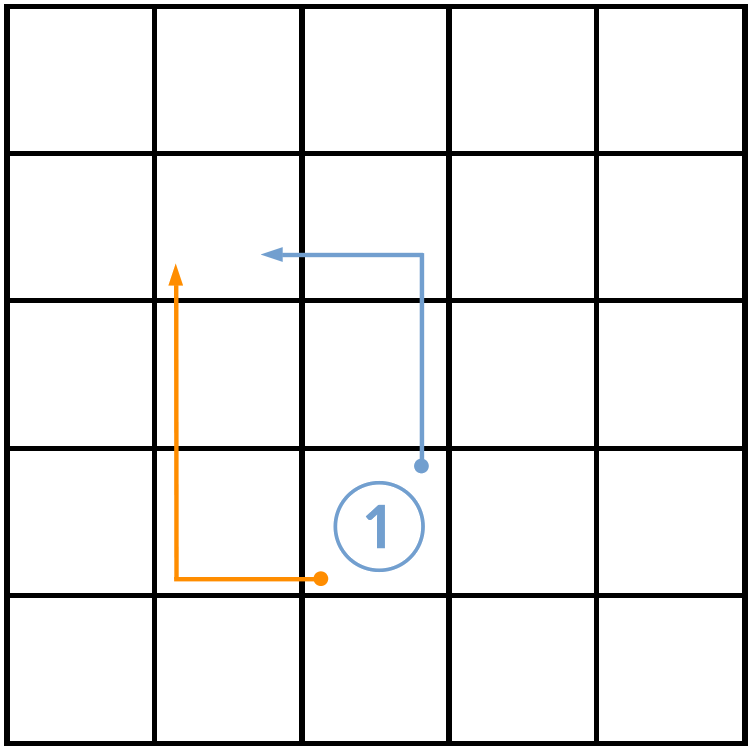
\includegraphics[width=200px]{images/manhattan_equal.png}
\end{figure}

\begin{figure}[h]
	\centering
	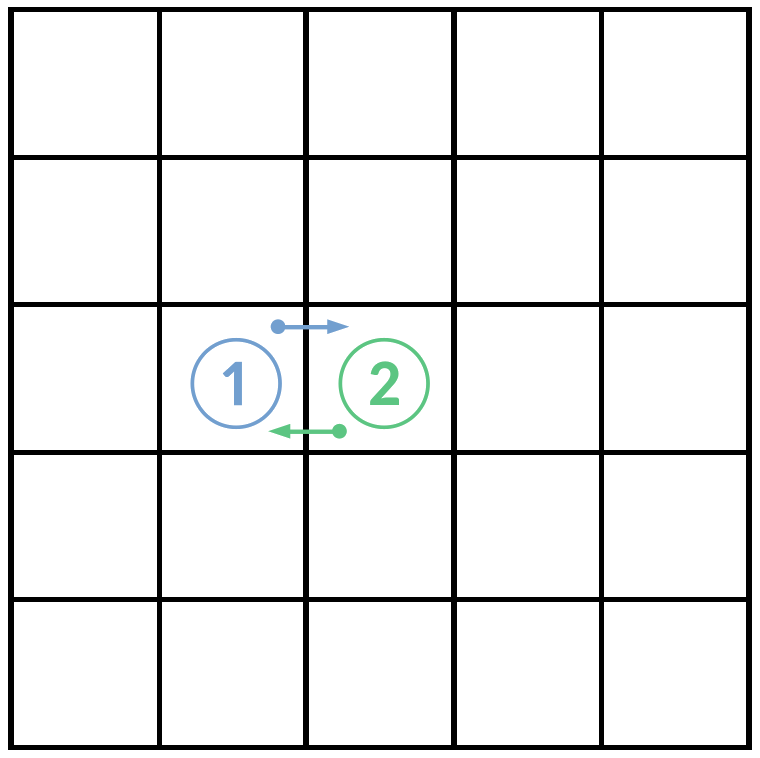
\includegraphics[width=200px]{images/switch.png}
\end{figure}

Contraites :

Chaque agent cognitif doit être doté de capacités de raisonnement et de réaction indépendantes, c'est le sens même de sa définition. Ici, chaque agent

\begin{figure}[h]
	\centering
	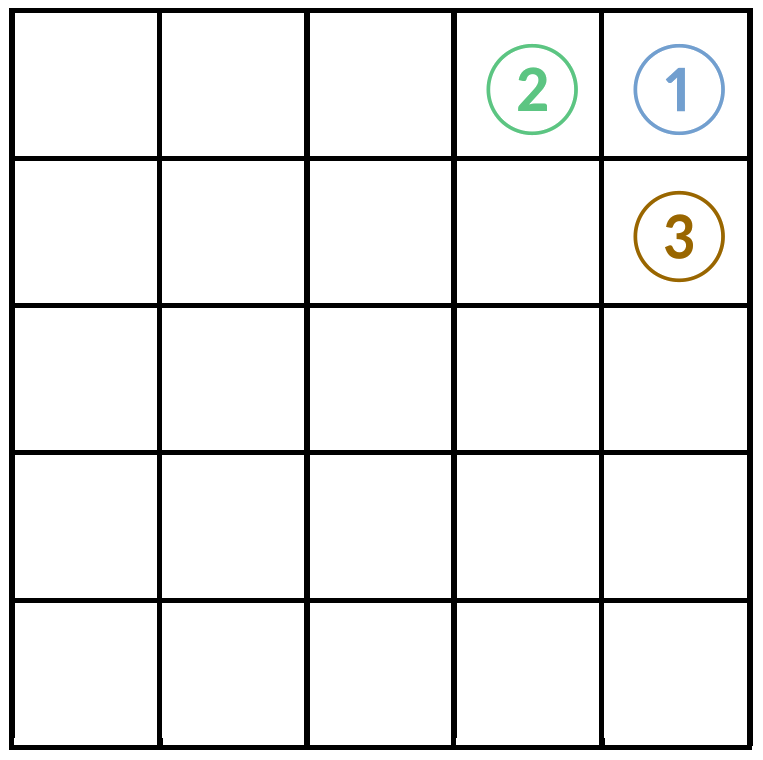
\includegraphics[width=200px]{images/3_agents.png}
\end{figure}

\begin{figure}[h]
	\centering
	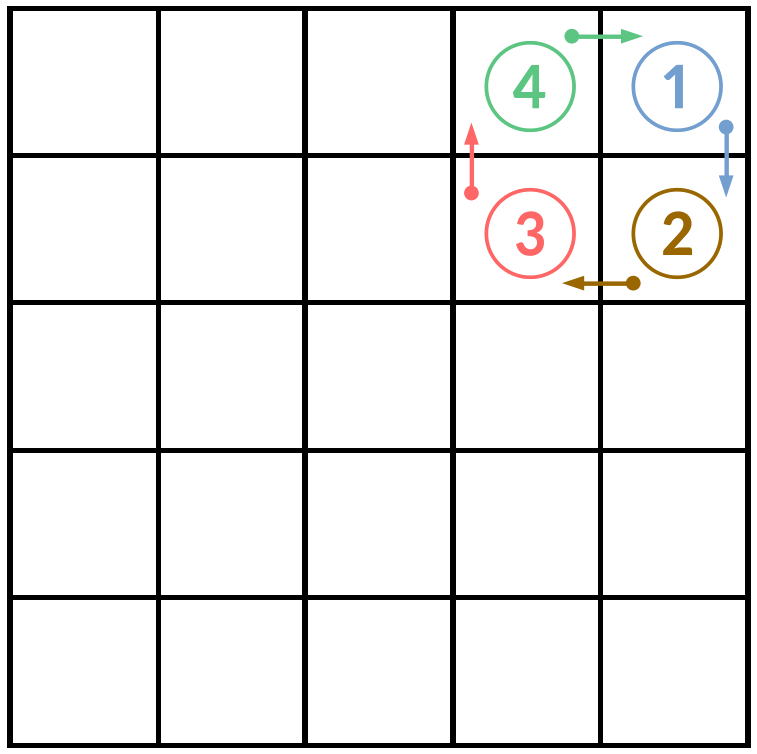
\includegraphics[width=200px]{images/4_agents.png}
\end{figure}

\end{document}
